\documentclass[10.5pt,a4paper]{article}
\usepackage[utf8]{inputenc}
\usepackage[T1]{fontenc}
\renewcommand{\contentsname}{Table des matières}
\usepackage{amsmath,amssymb}
\usepackage{geometry}
\geometry{margin=2cm}
\usepackage{tikz}
\usetikzlibrary{arrows.meta,calc}
\usepackage{xcolor}
\usepackage{enumitem}
\usepackage{booktabs}
\usepackage{longtable}
\usepackage{array}
\usepackage{tabularx}
\usepackage{mdframed}
\usepackage{hyperref}
\hypersetup{colorlinks=true,linkcolor=blue!50!black,urlcolor=blue}

\newmdenv[
  linecolor=violet!55!black, backgroundcolor=violet!5,
  linewidth=1pt, roundcorner=4pt, innermargin=8pt, innertopmargin=6pt, innerbottommargin=6pt,
  skipabove=8pt, skipbelow=8pt
]{objectif}

\newmdenv[
  linecolor=orange!70!black, backgroundcolor=orange!6,
  linewidth=1pt, roundcorner=4pt, innermargin=8pt, innertopmargin=6pt, innerbottommargin=6pt,
  skipabove=8pt, skipbelow=8pt
]{retenir}

% tableau ligne-par-ligne : colonne 1 = calcul (source du cours), colonne 2 = explication
\newenvironment{demotable}{%
\begin{longtable}{@{}>{\raggedright\arraybackslash}p{7.3cm} >{\raggedright\arraybackslash}p{8.3cm}@{}}
\toprule
\textbf{Étape (calcul)} & \textbf{Explication}\\
\midrule
\endfirsthead
\multicolumn{2}{l}{\small\itshape (suite)}\\[2pt]
\toprule
\textbf{Étape (calcul)} & \textbf{Explication}\\
\midrule
\endhead
\bottomrule
\endfoot
}{\end{longtable}}

\newcommand{\eqbox}[1]{\[\boxed{#1}\]}

\title{\textbf{Démonstrations à connaître -- Mécathermo}\\[4pt]\large Étape par étape, ligne par ligne}
\author{}
\date{}

\begin{document}
\maketitle
\vspace{-1cm}
\begin{center}
\small\itshape Chaque démonstration reprend le raisonnement du syllabus ligne par ligne, avec une explication
courte de ce qui se passe à chaque étape. Les numéros de diapositives cités sont ceux du syllabus.
\end{center}
\vspace{0.3cm}
\tableofcontents
\newpage

\section{Travail élémentaire réversible (diapos 34-40, dont 36-38)}

\begin{objectif}
\textbf{Objectif :} trouver une formule pour le travail échangé par un gaz qui se comprime ou se détend de
façon réversible (infiniment lente), à partir d'un simple bilan de forces sur un piston.
\end{objectif}

\begin{demotable}
$F = p\cdot S$ (état initial, piston à l'équilibre) &
Un piston de surface $S$ contenant un gaz à la pression $p$ subit une force $F=p\cdot S$ de la part du gaz.
Au départ le piston est à l'équilibre. \\
On augmente la force d'une quantité infinitésimale $dF$ ; le piston s'abaisse de $dl$ &
On pousse \emph{très légèrement} plus fort que l'équilibre (transformation réversible = infiniment lente) :
le piston bouge d'un tout petit déplacement $dl$. \\
$dW = |(F+dF)\cdot dl|$ &
Le travail élémentaire, c'est la force appliquée multipliée par le déplacement de son point d'application. \\
$dF$ négligeable devant $F$, donc $F+dF \approx F$ &
Comme $dF$ est infinitésimal, on peut le négliger \emph{dans le calcul de la force}, mais pas dans le
mouvement qu'il provoque. \\
$dW = |F\cdot dl| = |p\cdot S\cdot dl|$ &
On remplace $F$ par $p\cdot S$. \\
$dW>0$, $p>0$, $dl<0$ &
On regarde les signes : le travail reçu par le gaz lors d'une compression doit être positif ($dW>0$), la
pression est toujours positive, donc le déplacement $dl$ (compté positivement vers le haut) doit être
négatif (le piston descend, le gaz se comprime). \\
$dW = -p\cdot S\cdot dl$ &
Pour que $dW$ soit positif alors que $dl$ est négatif, il faut un signe $-$ devant. \\
$dW = -p\cdot dV$ &
$S\cdot dl$ est justement la variation élémentaire de volume $dV$ (surface $\times$ déplacement). C'est la
formule du \textbf{formulaire}. \\
\end{demotable}

\textbf{En intégrant} $dW=-p\,dV$ entre l'état initial $i$ et l'état final $f$ :
\eqbox{W = -\int_{V_i}^{V_f} p\,dV}

\begin{demotable}
Isochore : $dV=0$ &
Le volume ne varie pas $\Rightarrow$ $\boxed{W=0}$ (pas de déplacement du piston, pas de travail). \\
Isobare : $p=$ constante sort de l'intégrale &
$\boxed{W=-p\,(V_f-V_i)}$. \\
Isotherme, gaz parfait : $pV=nRT \Rightarrow p=\dfrac{nRT}{V}$ &
On remplace $p$ dans l'intégrale. \\
$W=-\displaystyle\int \frac{nRT}{V}\,dV = -nRT\int\frac{1}{V}\,dV$ &
$T$ est constante (isotherme) donc $nRT$ sort de l'intégrale ; il reste $\int \frac{1}{V}dV = \ln V$. \\
$\boxed{W = -nRT\,\ln\!\left(\dfrac{V_2}{V_1}\right)}$ &
Résultat de l'intégration entre $V_1$ et $V_2$. \\
\end{demotable}

\begin{retenir}
\textbf{Lecture d'un cycle sur un diagramme $p$-$V$ :} l'aire sous une courbe $=|W|$ de cette
transformation, et l'aire \emph{enfermée} par le cycle $=|W_{cycle}|$.

Pour un cycle parcouru dans le \textbf{sens horaire} : la \textbf{détente} se fait sur la partie
\textbf{haute} du cycle (à haute pression) et donne $W<0$ de grande valeur absolue ; la
\textbf{compression} se fait sur la partie \textbf{basse} (à basse pression) et ne coûte que $W>0$ plus
petit. La détente l'emporte donc $\Rightarrow$ $W_{cycle}<0$ : le cycle \textbf{fournit} du travail,
c'est un \textbf{cycle moteur}.

Parcouru en \textbf{sens antihoraire}, c'est l'inverse (on comprime à haute pression et on détend à basse
pression) $\Rightarrow$ $W_{cycle}>0$, le cycle \textbf{reçoit} du travail : c'est un \textbf{cycle
récepteur} (frigo, PAC).
\end{retenir}

\newpage
\section{Premier principe : énoncé et transformation entre deux points (diapos 41-49)}

\begin{demotable}
$\Delta U + \Delta E_{cin} + \Delta E_{pot} = W + Q$ &
Conservation de l'énergie : la variation de toute l'énergie du système (interne + cinétique + potentielle)
est égale à ce qu'il a reçu comme travail et comme chaleur. \\
$U$ : somme de l'énergie cinétique des particules et de l'énergie d'interaction entre elles, au niveau
microscopique &
C'est ce qu'on appelle l'énergie interne : toute l'agitation et les interactions invisibles à notre échelle. \\
$U$, $E_{cin}$, $E_{pot}$ sont des \textbf{fonctions d'état} ; $W$ et $Q$ \textbf{dépendent du chemin suivi} &
Une fonction d'état ne dépend que de l'état actuel du système (pas de comment on y est arrivé). $W$ et $Q$
dépendent, eux, de la transformation précise (réversible ou réelle) empruntée. \\
Pour un \textbf{cycle} (transformation fermée) : $U_i=U_f$, $E_{cin,i}=E_{cin,f}$, $E_{pot,i}=E_{pot,f}$ &
Dans un cycle, l'état final est identique à l'état initial (les états intermédiaires peuvent différer) donc
toutes les fonctions d'état reviennent à leur valeur de départ. \\
$\boxed{W+Q=0}$ pour un cycle &
Il ne reste que les termes qui dépendent du chemin ; leur somme sur le cycle complet doit être nulle. \\
\end{demotable}

\textbf{Ce qui se passe entre deux points A et B (raisonnement du cours) :} on prend un cycle A$\to$B via
un chemin $a$, puis B$\to$A via un chemin $c$ (c'est un cycle, donc $W_a+Q_a+W_c+Q_c=0$). On refait pareil
avec un autre chemin $b$ pour aller de A à B : $W_b+Q_b+W_c+Q_c=0$. En comparant les deux lignes, le terme
$W_c+Q_c$ (commun) disparaît :
\eqbox{W_a+Q_a = W_b+Q_b}

\begin{retenir}
\textbf{Conclusion (diapo 49) :} si on ne regarde \emph{que} la transformation ouverte de A vers B (sans le
retour), la somme $W+Q$ est \textbf{la même quel que soit le chemin suivi} entre ces deux points -- que ce
chemin soit réversible ou réel. Cela confirme que $W+Q=\Delta U+\Delta E_{cin}+\Delta E_{pot}$ ne dépend que
des points de départ et d'arrivée, jamais du trajet.
\end{retenir}

\newpage
\section{Premier principe en machine ouverte (diapos 65-72, dont 68-73)}

\begin{objectif}
\textbf{Objectif :} dans un compresseur, une turbine, une pompe... le fluide \emph{traverse} la machine en
continu. On veut une formule utilisable pour le \textbf{travail utile} $W_{ut}$ réellement échangé avec
l'arbre de la machine (et pas le travail «perdu» à pousser le fluide devant et derrière soi).
\end{objectif}

\textbf{Hypothèses :} régime permanent (le débit massique et les grandeurs physiques ne varient pas dans le
temps), fluide parfait (pas d'interactions entre molécules), transformation réversible.

\textbf{Schéma :} on suit une tranche de fluide de masse $M$, comprise entre les sections $S_a,S_b$ à
l'instant $t$ (entrée à pression $p_1$, volume $V_1$) et entre $S'_a,S'_b$ à l'instant $t+\Delta t$ (sortie
à pression $p_2$, volume $V_2$).

\begin{demotable}
$W_t = W_{ut} - p_2V_2 + p_1V_1$ &
Le travail total des forces extérieures sur la tranche de fluide = le travail utile donné par la machine
$\pm$ le travail des pressions d'entrée/sortie : $p_1V_1$ est le travail que le fluide \emph{derrière}
pousse sur notre tranche (il la fait avancer, énergie reçue), $p_2V_2$ est le travail que notre tranche doit
fournir pour pousser le fluide \emph{devant} elle (énergie cédée). \\
1\textsuperscript{er} principe sur $M$ pendant $\Delta t$ :
$U_2-U_1+\Delta E_{cin}+\Delta E_{pot} = W_{ut}-p_2V_2+p_1V_1+Q$ &
On applique simplement $\Delta U+\Delta E_{cin}+\Delta E_{pot}=W+Q$ en remplaçant $W$ par l'expression du
travail total trouvée juste au-dessus. \\
$(U_2+p_2V_2)-(U_1+p_1V_1)+\Delta E_{cin}+\Delta E_{pot}=W_{ut}+Q$ &
On regroupe les termes en $p_1V_1$ et $p_2V_2$ avec les $U$ correspondants. \\
$\boxed{\Delta H+\Delta E_{cin}+\Delta E_{pot}=W_{ut}+Q}$ &
On reconnaît $U+pV=H$ (l'enthalpie) en 1 et en 2. C'est la version «machine ouverte» du 1\textsuperscript{er}
principe -- à comparer avec $\Delta U=W+Q$ en système fermé. \\
Par unité de masse : $dh+\dfrac{c^2}{2}+g\,\Delta z = w_{ut}+q$ &
Même relation, en divisant tout par la masse (c = vitesse du fluide, $\Delta z$ = variation d'altitude). \\
\end{demotable}

\textbf{Isoler $W_{ut}$} (cas où $\Delta E_{cin}=\Delta E_{pot}=0$, on repart de la même équation) :

\begin{demotable}
$W_{ut}-p_2V_2+p_1V_1+Q = W_{ut}-\Delta(pV)+Q = W_{ut}-\displaystyle\int_1^2 d(pV)+Q$ &
$p_2V_2-p_1V_1$ est la variation de la fonction $pV$ entre 1 et 2, qu'on peut écrire comme une intégrale. \\
$= W_{ut}-\displaystyle\int_1^2 p\,dV-\int_1^2 V\,dp+Q$ &
On utilise la règle de dérivation d'un produit : $d(pV)=p\,dV+V\,dp$. \\
$U_2-U_1=W_{ut}-\displaystyle\int_1^2 p\,dV-\int_1^2 V\,dp+Q$ &
On réinjecte ceci dans le 1\textsuperscript{er} principe de départ. \\
Or, pour la même tranche : $\Delta U=W_t+Q$ et $W_t=-\displaystyle\int p\,dV$
$\Rightarrow \Delta U - Q=-\displaystyle\int p\,dV$ &
On utilise une deuxième expression de $\Delta U$, celle d'un système fermé classique (le travail des forces
de pression «normales» sur la tranche). \\
$W_{ut}=\displaystyle\int_1^2 p\,dV+\int_1^2 V\,dp-\int_1^2 p\,dV$ &
On combine les deux expressions de $U_2-U_1$ : les termes en $\int p\,dV$ et $Q$ s'annulent des deux côtés. \\
$\boxed{W_{ut}=\displaystyle\int_1^2 V\,dp}$ \quad (si $\Delta E_{cin}=\Delta E_{pot}=0$) &
C'est le résultat central : le travail utile d'un compresseur/turbine se calcule avec $\int V\,dp$, \textbf{pas}
avec $\int p\,dV$ (qui, lui, ne concerne que les systèmes fermés). \\
Cas général : $\boxed{W_{ut}=\displaystyle\int_1^2 V\,dp+\dfrac{mc^2}{2}+mg\,\Delta z}$ &
On rajoute les termes cinétique et potentiel si on ne peut pas les négliger. \\
Fluide réel (avec frottements) : $\boxed{W_{ut}=\displaystyle\int_1^2 V\,dp+\dfrac{mc^2}{2}+mg\,\Delta z+W_f}$,
$W_f>0$ &
Les frottements (entre particules, ou entre le fluide et les parois) coûtent toujours de l'énergie
supplémentaire, on l'ajoute avec un signe $+$. \\
\end{demotable}

\newpage
\section{Chaleurs spécifiques massique et molaire (diapos 73-76, dont 75-77)}

\begin{objectif}
\textbf{Objectif :} relier la chaleur spécifique $C_v$ et $C_p$ (que l'on utilise tout le temps dans les
exercices) à l'énergie interne $U$ et à l'enthalpie $H$.
\end{objectif}

\textbf{Définitions} : $c=\dfrac{1}{m}\cdot\dfrac{dQ}{dT}$ [J/(kg·K)] (chaleur spécifique \textbf{massique})
et $C=\dfrac{1}{n}\cdot\dfrac{dQ}{dT}$ [J/(mol·K)] (chaleur spécifique \textbf{molaire}), avec $C=M\cdot c$
($M$ = masse molaire). \emph{En mots :} c'est la quantité de chaleur qu'il faut apporter pour élever d'1 K
la température d'1 kg (ou d'1 mole) de matière.

\begin{demotable}
1\textsuperscript{er} principe : $dU=dQ+dW=dQ-p\,dV \Rightarrow dQ=dU+p\,dV$ &
On part du 1\textsuperscript{er} principe pour exprimer $dQ$ (on utilise $dW=-p\,dV$, réversible). \\
$C=\dfrac{1}{n}\cdot\dfrac{dQ}{dT}=\dfrac{1}{n}\left(\dfrac{dU}{dT}+p\dfrac{dV}{dT}\right)$ &
On remplace $dQ$ par l'expression trouvée. C'est la formule \textbf{générale}, valable pour n'importe
quelle transformation. \\
Volume constant : $\boxed{C_v=\dfrac{1}{n}\cdot\dfrac{dU}{dT}}$ &
Si $V$ est constant, $dV=0$ : le deuxième terme disparaît complètement. \\
Pression constante : $C_p=\dfrac{1}{n}\left(\dfrac{dU}{dT}+p\dfrac{dV}{dT}+V\dfrac{dp}{dT}\right)$ &
\textbf{Astuce du cours} : on \emph{ajoute} le terme $V\dfrac{dp}{dT}$, qui vaut $0$ puisque $p$ est
constant ($dp=0$) -- cela ne change donc rien à l'équation, mais permet de compléter une dérivée de produit. \\
$=\dfrac{1}{n}\left(\dfrac{dU}{dT}+\dfrac{d(pV)}{dT}\right)=\dfrac{1}{n}\cdot\dfrac{d(U+pV)}{dT}$ &
On reconnaît la règle du produit $\dfrac{d(pV)}{dT}=p\dfrac{dV}{dT}+V\dfrac{dp}{dT}$, ce qui permet de
regrouper les deux termes. \\
$\boxed{C_p=\dfrac{1}{n}\cdot\dfrac{dH}{dT}}$ &
$U+pV=H$ par définition de l'enthalpie. \\
\end{demotable}

\textbf{Dans l'autre sens} (utile pour les calculs) : de $C_v=\frac{1}{n}\frac{dU}{dT}$ on tire directement
$dU=nC_v\,dT$ -- \emph{cette relation est toujours vraie pour un gaz parfait}, quelle que soit la
transformation, car $U$ ne dépend que de $T$. À volume constant, $W=0$, donc en plus
$\boxed{dQ=dU=nC_v\,dT}$. De même $dH=nC_p\,dT$ est toujours vrai, et à pression constante $W_{ut}=0$
donc $\boxed{dQ=dH=nC_p\,dT}$.

\begin{demotable}
\textbf{Relation de Mayer} : $C_p=\dfrac{1}{n}\dfrac{dU}{dT}+\dfrac{1}{n}\dfrac{d(pV)}{dT}$
$=C_v+\dfrac{1}{n}\dfrac{d(nRT)}{dT}$ &
On repart de la définition de $C_p$ et on utilise $pV=nRT$ (gaz parfait) pour le deuxième terme. \\
$=C_v+\dfrac{1}{n}\cdot n\cdot R$ &
$n$ et $R$ sont des constantes, la dérivée de $nRT$ par rapport à $T$ vaut simplement $nR$. \\
$\boxed{C_p-C_v=R}$ (ou $c_p-c_v=R/M$ en massique) &
On isole. C'est la relation de Mayer, dans le \textbf{formulaire}. \\
$C_p>C_v$, on pose $\dfrac{C_p}{C_v}=\gamma>1$ ($\gamma=1{,}4$ pour l'air) &
Puisque $R>0$, $C_p$ est toujours plus grand que $C_v$ : il faut plus de chaleur pour chauffer un gaz à
pression constante (une partie sert à le dilater) qu'à volume constant. \\
\end{demotable}

\newpage
\section{Transformation adiabatique réversible (diapos 77-84, dont 80-83)}

\begin{objectif}
\textbf{Objectif :} trouver la relation entre $p$, $V$ et $T$ pour une compression/détente
\textbf{rapide} (pas le temps d'échanger de la chaleur) et \textbf{réversible}. C'est la formule la plus
utilisée du cours (moteurs, compresseurs, turbines).
\end{objectif}

\subsection*{Démonstration de la 1\textsuperscript{ère} formule : $T\,V^{\gamma-1}=$ constante}

\begin{demotable}
Adiabatique $\Rightarrow dQ=0$, donc $dW=dU$ &
Par définition, une transformation adiabatique n'échange pas de chaleur ; le 1\textsuperscript{er} principe
$dU=dW+dQ$ se réduit à $dU=dW$. \\
Réversible $\Rightarrow dW=-p\,dV$, et gaz parfait $\Rightarrow dU=nC_v\,dT$ &
On utilise le travail élémentaire réversible (section 1) et la relation $dU=nC_v\,dT$ toujours valable pour
un gaz parfait. \\
$nC_v\,dT+p\,dV=0$ &
On combine les deux lignes précédentes ($dU=dW \Rightarrow nC_v\,dT=-p\,dV$, on réarrange). \\
Gaz parfait : $pV=nRT \Rightarrow p=\dfrac{nRT}{V}$, donc $nC_v\,dT+nRT\dfrac{dV}{V}=0$ &
On remplace $p$ pour n'avoir plus que $T$ et $V$ dans l'équation. \\
$\boxed{C_v\dfrac{dT}{T}+R\dfrac{dV}{V}=0}$ &
On divise toute l'équation par $n$ puis par $T$, pour faire apparaître des rapports «logarithmiques»
($dT/T$ et $dV/V$). \\
On divise par $C_v$ et on utilise $\dfrac{R}{C_v}=\dfrac{C_p-C_v}{C_v}=\gamma-1$ &
On veut faire apparaître $\gamma$ ; comme $C_p-C_v=R$ et $C_p/C_v=\gamma$, on a $R/C_v=\gamma-1$. \\
$\dfrac{dT}{T}+(\gamma-1)\dfrac{dV}{V}=0$ &
Équation réécrite uniquement avec $\gamma$. \\
Intégration : $\ln(T)+(\gamma-1)\ln(V)=$ constante &
$\int \frac{dT}{T}=\ln T$ et $\int\frac{dV}{V}=\ln V$ ; la somme des deux primitives reste une constante. \\
On applique l'exponentielle des deux côtés &
$e^{\ln T + (\gamma-1)\ln V}=e^{\text{constante}}$, ce qui simplifie les logarithmes. \\
$\boxed{T\cdot V^{\gamma-1}=\text{constante}}$ &
Résultat final : c'est la 1\textsuperscript{ère} formule de l'adiabatique réversible. \\
\end{demotable}

\subsection*{Comment obtenir les 2 autres formules (par substitution, avec $pV=nRT$)}

\begin{demotable}
En fonction de $p$ et $V$ : on remplace $T=\dfrac{pV}{nR}$ dans $T\,V^{\gamma-1}=$ cste &
On veut éliminer $T$ au profit de $p$ : on utilise simplement la loi des gaz parfaits pour l'exprimer. \\
$\dfrac{pV}{nR}\cdot V^{\gamma-1}=$ cste $\Rightarrow \dfrac{p\,V^{\gamma}}{nR}=$ cste &
On regroupe les puissances de $V$ ($V\cdot V^{\gamma-1}=V^\gamma$). \\
$n R$ est constant, on l'absorbe dans la constante &
$n$ (quantité de matière) et $R$ ne changent pas pendant la transformation, donc $p\,V^\gamma/(nR)=$cste
$\Leftrightarrow p\,V^\gamma=$ une autre constante. \\
$\boxed{p\,V^\gamma=\text{constante}}$ &
2\textsuperscript{ème} formule, celle utilisée pour lire un diagramme $p$-$V$. \\
\midrule
En fonction de $T$ et $p$ : on remplace $V=\dfrac{nRT}{p}$ dans $T\,V^{\gamma-1}=$ cste &
Même logique, mais on élimine $V$ cette fois. \\
$T\cdot\left(\dfrac{nRT}{p}\right)^{\gamma-1}=$ cste $\Rightarrow T\cdot(nR)^{\gamma-1}\cdot T^{\gamma-1}\cdot
p^{-(\gamma-1)}=$ cste &
On développe la puissance $(\gamma-1)$ sur chaque facteur de la fraction. \\
$T^{\gamma}\cdot p^{-(\gamma-1)}=\dfrac{\text{cste}}{(nR)^{\gamma-1}}$, et $(nR)^{\gamma-1}$ est constant &
On regroupe les puissances de $T$ ($T\cdot T^{\gamma-1}=T^\gamma$) et on absorbe le facteur constant
restant. \\
$\boxed{T^{\gamma}\cdot p^{1-\gamma}=\text{constante}}$ &
3\textsuperscript{ème} formule. Les trois formes sont \textbf{équivalentes} : on choisit celle qui utilise
les variables connues dans l'exercice. \\
\end{demotable}

\begin{retenir}
En dérivant $pV=$cste (isotherme) et $pV^\gamma=$cste (adiabatique) on trouve les pentes
$\frac{dp}{dV}=-\frac{p}{V}$ (isotherme) et $\frac{dp}{dV}=-\frac{p\gamma}{V}$ (adiabatique). Comme
$\gamma>1$, \textbf{une adiabatique est toujours plus pentue qu'une isotherme passant par le même point.}
\end{retenir}

\newpage
\section{Réversible vs irréversible : ce qui se passe, et calcul de $Q$ et $W$ (diapos 91-93)}

\begin{objectif}
\textbf{Objectif :} montrer qu'une transformation \textbf{irréversible} coûte toujours \textbf{plus de
travail} pour obtenir \textbf{moins de chaleur} qu'une transformation réversible entre les deux mêmes états.
C'est la base de tous les rendements du cours (rien n'est jamais parfait).
\end{objectif}

\textbf{Rappel (transformation fermée monotherme, diapo 91) :} le second principe impose $\Delta W\geq0$.
Si la transformation est réversible, la seule possibilité est $\Delta W=0$ et $\Delta Q=0$ ; si elle est
irréversible, la seule possibilité est $\Delta W>0$ et $\Delta Q<0$ (il faut fournir du travail net et on
perd de la chaleur).

\subsection*{Cas de deux transformations réversibles I et II (diapo 92)}
\begin{demotable}
On observe la transformation totale $I+(-II)$ (aller par I, revenir par II en sens inverse) &
C'est un \textbf{cycle fermé monotherme réversible} (composé de deux morceaux réversibles). \\
$W_{tot}=0=W_I+W_{-II}=0 \Rightarrow \boxed{W_I=W_{II}}$ &
D'après le rappel ci-dessus, un cycle fermé monotherme réversible a $\Delta W=0$. Donc les deux chemins
réversibles I et II demandent exactement le \textbf{même travail}. \\
$W_I+Q_I=W_{II}+Q_{II}=\Delta U \Rightarrow \boxed{Q_I=Q_{II}}$ &
Comme $W_I=W_{II}$, l'égalité $\Delta U=W+Q$ (même $\Delta U$ car même trajet A$\to$B) impose aussi
$Q_I=Q_{II}$. \\
\end{demotable}

\subsection*{Cas où I est irréversible et II reste réversible (diapo 93)}
\begin{demotable}
$W_{tot}>0 \Rightarrow W_I+W_{-II}>0 \Rightarrow \boxed{W_I>W_{II}}$ &
Cette fois le cycle total $I+(-II)$ contient une partie irréversible, donc $\Delta W>0$ (rappel plus haut) :
le travail du chemin irréversible I est \textbf{plus grand} que celui du chemin réversible II. \\
$\boxed{W_{\text{irréversible}}>W_{\text{réversible}}}$ et donc $\boxed{Q_{\text{irréversible}}<Q_{\text{réversible}}}$ &
Puisque $\Delta U$ est le même (mêmes points de départ/arrivée) et que $W+Q=\Delta U$ est fixe, si $W$
augmente alors $Q$ doit diminuer d'autant. \\
\end{demotable}

\begin{retenir}
\textbf{Ce qu'il se passe physiquement :} en irréversible, une partie de l'énergie fournie est «gaspillée» (frottements, pertes de charge, combustion non instantanée...). Il faut donc \textbf{fournir un
travail plus important} pour obtenir, au final, \textbf{une quantité de chaleur plus petite} que si la
même transformation avait pu se faire de façon réversible. C'est exactement ce qui justifie les rendements
$\eta_f$, $\eta_{\text{méca}}$ du cours sur les moteurs, et les $\eta_{isos}$ des compresseurs frigo.
\end{retenir}

\newpage
\section{Cycle de Carnot : courbes utilisées et démonstration du rendement (diapos 103-108)}

\begin{objectif}
\textbf{Objectif :} calculer le meilleur rendement \textbf{possible} pour un moteur thermique fonctionnant
entre deux sources de chaleur -- c'est la limite théorique absolue, jamais atteinte en pratique.
\end{objectif}

\textbf{Les 4 courbes du cycle de Carnot} (les deux seules formes de transformation qui n'engendrent
\textbf{aucune irréversibilité}) :
\begin{itemize}[leftmargin=1.4em]
\item A$\to$B : \textbf{compression adiabatique réversible} ($Q=0$, $W>0$)
\item B$\to$C : \textbf{détente isotherme réversible} ($Q>0$, $W<0$) -- la source chaude $T_1$ fournit $Q_1$
\item C$\to$D : \textbf{détente adiabatique réversible} ($Q=0$, $W<0$)
\item D$\to$A : \textbf{compression isotherme réversible} ($Q<0$, $W>0$) -- la source froide $T_2$ reçoit
$Q_2$
\end{itemize}
\emph{En mots :} on comprime et détend le gaz sans jamais échanger de chaleur pendant les phases rapides
(adiabatiques), et on échange toute la chaleur pendant les phases lentes à température constante
(isothermes) -- c'est ce qui rend le cycle totalement réversible.

\begin{demotable}
$\eta=\dfrac{\text{énergie utile}}{\text{énergie fournie}}=\dfrac{|W_{tot}|}{Q_1}=\dfrac{|-Q_1-Q_2|}{Q_1}$ &
Le rendement, c'est toujours ce qu'on récupère (le travail net) divisé par ce qu'on a dû payer
(la chaleur $Q_1$ fournie par la source chaude). $W_{tot}=-Q_1-Q_2$ vient de $\Delta U_{cycle}=0=Q_1+Q_2+W_{tot}$. \\
$\eta=\dfrac{Q_1+Q_2}{Q_1}=\boxed{1+\dfrac{Q_2}{Q_1}}$ \quad ($W_{tot}<0$ car machine motrice) &
On simplifie la valeur absolue car $W_{tot}$ est négatif pour un cycle moteur. \\
Comme $Q_2<0$ et $|Q_2|<|Q_1|$ : $0\leq\eta<1$ &
$Q_2/Q_1$ est négatif mais de valeur absolue $<1$, donc $\eta$ reste entre 0 et 1 : jamais 100\%. \\
Sur une isotherme, $\Delta U=0 \Rightarrow Q=-W=-nRT\ln\!\left(\dfrac{V_i}{V_f}\right)$ &
Pour calculer $Q_1$ et $Q_2$ explicitement, on utilise le travail d'une isotherme (section 1) et le fait
que $Q=-W$ quand $\Delta U=0$. \\
$\eta=1+\dfrac{Q_{DA}}{Q_{BC}}=1-\dfrac{T_A\ln(V_A/V_D)}{T_C\ln(V_B/V_C)}$ &
On applique la formule ci-dessus aux deux isothermes B-C (à $T_C$) et D-A (à $T_A$) ; les $Q_1,Q_2$
deviennent des logarithmes de rapports de volumes. \\
Relations adiabatiques : $T_AV_A^{\gamma-1}=T_BV_B^{\gamma-1}$ (A-B) et $T_CV_C^{\gamma-1}=T_DV_D^{\gamma-1}$
(C-D), avec $T_B=T_C$ et $T_D=T_A$ &
On utilise la 1\textsuperscript{ère} formule de l'adiabatique (section 2) sur les deux portions adiabatiques
du cycle, en notant que B et C sont à la même température (idem D et A, isothermes). \\
$\left(\dfrac{V_A}{V_B}\right)^{\gamma-1}=\dfrac{T_B}{T_A}=\dfrac{T_C}{T_D}=\left(\dfrac{V_D}{V_C}\right)^{\gamma-1}
\Rightarrow \dfrac{V_A}{V_B}=\dfrac{V_D}{V_C} \Rightarrow \boxed{\dfrac{V_A}{V_D}=\dfrac{V_B}{V_C}}$ &
En combinant les 4 relations, on montre que les deux rapports de volumes sont \textbf{égaux} -- c'est
l'étape clé : cela va faire disparaître les logarithmes de volume dans le rendement ! \\
Donc $\ln(V_A/V_D)=\ln(V_B/V_C)$, ces deux termes se simplifient dans la fraction &
Puisque les rapports sont égaux, leurs logarithmes le sont aussi : la fraction $\frac{\ln(V_A/V_D)}{\ln(V_B/V_C)}$
vaut exactement $1$. \\
$\boxed{\eta_{Carnot}=1-\dfrac{T_A}{T_C}}$ &
Il ne reste que le rapport des températures. Avec $T_A=T_2$ (froide) et $T_C=T_1$ (chaude), c'est la formule
$\eta_{Carnot}=1-T_2/T_1$ du \textbf{formulaire}. \\
\end{demotable}

\begin{retenir}
Même dans ce cas théorique \textbf{parfait} (aucune irréversibilité), le rendement n'est jamais égal à 1 :
il ne dépend que du rapport des deux températures des sources. C'est la limite indépassable pour
\textbf{tout} moteur thermique ditherme, quel que soit le fluide ou la technologie utilisée.
\end{retenir}

\newpage
\section{Cycle de Joule (turbine à gaz) : démonstration et utilisation (diapos 109-116)}

\subsection*{Le cycle fermé théorique (diapos 109-112)}

\textbf{Les 4 transformations} (même schéma logique que Carnot, mais avec des \textbf{isobares} à la place
des isothermes -- plus simple à réaliser techniquement, mais irréversibles) :
\begin{itemize}[leftmargin=1.4em]
\item A$\to$B : compression \textbf{adiabatique réversible} ($Q=0$, $W>0$)
\item B$\to$C : détente \textbf{isobare irréversible} ($Q>0$, $W<0$) -- la source chaude $T_1$ fournit $Q_1$
\item C$\to$D : détente \textbf{adiabatique réversible} ($Q=0$, $W<0$)
\item D$\to$A : compression \textbf{isobare irréversible} ($Q<0$, $W>0$) -- la source froide $T_2$ reçoit
$Q_2$
\end{itemize}

\begin{demotable}
$\eta=1+\dfrac{Q_2}{Q_1}=1+\dfrac{Q_{DA}}{Q_{BC}}=1+\dfrac{nC_p(T_A-T_D)}{nC_p(T_C-T_B)}$ &
Même point de départ que Carnot ($\eta=1+Q_2/Q_1$), mais ici les échanges de chaleur se font à
\textbf{pression constante} : on utilise donc $Q=nC_p\Delta T$ au lieu de la formule isotherme. \\
Relations adiabatiques (A-B et C-D) : $T_Ap_A^{(\gamma-1)/\gamma}=T_Bp_B^{(\gamma-1)/\gamma}$ et
$T_Dp_D^{(\gamma-1)/\gamma}=T_Cp_C^{(\gamma-1)/\gamma}$, avec $p_A=p_D$ et $p_B=p_C$ (isobares) &
On utilise la 3\textsuperscript{ème} formule de l'adiabatique ($T^\gamma p^{1-\gamma}=$cste) sur les deux
portions adiabatiques ; les pressions se correspondent car B-C et D-A sont isobares. \\
$\Rightarrow \dfrac{T_A}{T_D}=\dfrac{T_B}{T_C}=\dfrac{T_A-T_D}{T_B-T_C}=-\dfrac{T_A-T_D}{T_C-T_B}$ &
En combinant les deux relations (même astuce que pour Carnot : deux rapports égaux $\Rightarrow$ leur
différence donne le même rapport), on relie directement les 4 températures. \\
$\boxed{\eta_J=1-\dfrac{T_A}{T_B}}$ &
Les $(T_A-T_D)$ se simplifient avec ceux du rendement, il ne reste que $T_A$ et $T_B$. \\
Comparaison à Carnot : $\eta_{Carnot}=1-\dfrac{T_A}{T_C}$, or $T_C>T_B$ &
$T_C$ est la température atteinte après la détente isobare complète, $T_B$ seulement après la compression :
$T_C>T_B$ toujours. \\
$\boxed{\eta_{Carnot}>\eta_{Joule}}$ &
Puisque $T_C>T_B$, diviser $T_A$ par $T_C$ donne un nombre plus petit que diviser $T_A$ par $T_B$ : le
rendement de Joule est \textbf{plus bas} que celui de Carnot, car les isobares ne sont pas réversibles. \\
\end{demotable}

\subsection*{Utilisation : le cycle de Joule ouvert (groupe électrogène / turboréacteur, diapos 113-116)}

\textbf{En pratique}, on ne referme pas le cycle : un compresseur axial (entraîné par la turbine, sur le
même arbre) aspire de l'air frais en A, l'air ressort comprimé en B, est chauffé dans la chambre de
combustion (injection de carburant, $Q_1$) jusqu'en C, puis se détend dans la turbine jusqu'en D en
ressortant sous forme de gaz brûlés (remplacés par de l'air neuf en A au cycle suivant -- \textbf{cycle
ouvert}). \textbf{Une grande partie du travail récupéré à la détente sert directement à entraîner le
compresseur.}

\begin{demotable}
$\eta=\dfrac{-W_{ut}}{Q_1}=\dfrac{-(W_{CD}-W_{AB})}{Q_{BC}}$, avec $Q_{BC}=H_C-H_B=nC_p(T_C-T_B)$ &
Ici les machines sont \textbf{ouvertes} (compresseur, turbine) : on utilise le rendement basé sur
$W_{ut}$, et $Q_{BC}$ (isobare) se calcule avec l'enthalpie, comme pour tout échangeur ouvert. \\
Machine ouverte adiabatique : $H_f-H_i=W_{ut}+Q$ et $Q=0 \Rightarrow W_{ut}=\Delta H$ &
Résultat de la section 1 (machine ouverte) appliqué aux étapes adiabatiques A-B et C-D : pas de chaleur
échangée, donc tout le travail utile = variation d'enthalpie. \\
$W_{CD}=H_D-H_C$ et $W_{AB}=H_B-H_A$ &
On applique ce résultat spécifiquement aux deux détentes/compressions adiabatiques du cycle. \\
$\eta=\dfrac{-H_D+H_C-H_B+H_A}{H_C-H_B}$, et $\Delta H=nC_p\Delta T$ &
On remplace $W_{CD}$ et $W_{AB}$ par leurs expressions en $H$, puis on repasse en températures. \\
$\boxed{\eta=1+\dfrac{-T_D+T_A}{T_C-T_B}}$ &
Même résultat que la version fermée (à une réécriture près) : la démonstration par les enthalpies confirme
le résultat obtenu avec les températures. \\
\end{demotable}

\newpage
\section{Moteur essence (Beau de Rochas) : cycle, rendement, puissance (diapos 133-146)}

\subsection*{Le cycle en 4 temps -- ce qui se passe physiquement}
\begin{demotable}
\textbf{1. Admission} (A$\to$B, isobare) &
La soupape d'admission s'ouvre, le piston descend du PMH au PMB en aspirant un mélange air+carburant, à
pression constante ($p_{atm}$). \\
\textbf{2. Compression} (B$\to$C, \textbf{adiabatique}) &
Soupapes fermées, compression rapide : le système de refroidissement n'a pas le temps d'évacuer la
chaleur, donc $Q\approx0$. \\
\textbf{3. Explosion + détente} (C$\to$D isochore, puis D$\to$E adiabatique) &
La bougie déclenche l'explosion au point C : augmentation \textbf{quasi instantanée} de pression à volume
constant (C-D), puis détente adiabatique (D-E) qui pousse le piston -- c'est le \textbf{temps moteur}. \\
\textbf{4. Échappement} (E$\to$B isochore, puis B$\to$A isobare) &
La soupape d'échappement s'ouvre : chute de pression à volume constant (E-B) puis expulsion des gaz brûlés
lors de la remontée du piston (B-A), à pression constante. \\
\end{demotable}

\begin{center}
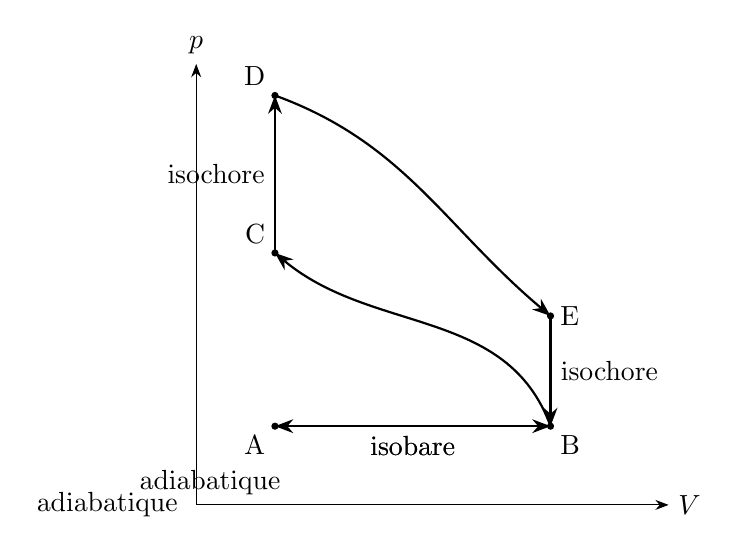
\begin{tikzpicture}[scale=1, >=Stealth]
\draw[->] (0,0) -- (6,0) node[right] {$V$};
\draw[->] (0,0) -- (0,5.6) node[above] {$p$};
\coordinate (A) at (1,1); \coordinate (B) at (4.5,1);
\coordinate (C) at (1,3.2); \coordinate (D) at (1,5.2);
\coordinate (E) at (4.5,2.4);
\draw[thick,->] (A) -- (B) node[midway,below]{isobare};
\draw[thick,->] (B) to[out=110,in=-40] (C) node[midway,left,xshift=-3pt]{adiabatique};
\draw[thick,->] (C) -- (D) node[midway,left]{isochore};
\draw[thick,->] (D) to[out=-20,in=140] (E) node[midway,above,xshift=5pt]{adiabatique};
\draw[thick,->] (E) -- (B) node[midway,right]{isochore};
\draw[thick,dashed,->] (B) -- (A) node[midway,below]{isobare};
\foreach \p/\lab/\pos in {A/A/below left,B/B/below right,C/C/above left,D/D/above left,E/E/right}
  {\fill (\p) circle (1.3pt) node[\pos] {\lab};}
\end{tikzpicture}
\end{center}

\begin{retenir}
En réalité, seul le \textbf{cycle utile B-C-D-E-B} compte pour le rendement : l'admission (A-B) et
l'échappement (B-A) sont sur la \textbf{même isobare}, parcourue en sens opposé, donc leur travail s'annule
exactement sur un cycle complet.
\end{retenir}

\subsection*{Démonstration du rendement théorique}
\begin{demotable}
$\eta=1+\dfrac{Q_{EB}}{Q_{CD}}=1+\dfrac{nC_v(T_B-T_E)}{nC_v(T_D-T_C)}$ &
Même logique que Carnot : rendement $=1+\frac{\text{chaleur perdue}}{\text{chaleur reçue}}$. Ici les deux
échanges de chaleur sont isochores, donc $Q=nC_v\Delta T$. \\
Adiabatiques B-C et D-E : $T_BV_B^{\gamma-1}=T_CV_C^{\gamma-1}$ et $T_EV_E^{\gamma-1}=T_DV_D^{\gamma-1}$, avec
$V_E=V_B$ et $V_D=V_C$ (isochores) &
On applique la formule de l'adiabatique aux deux détentes/compressions. Comme la combustion (C-D) et
l'échappement (E-B) sont à volume constant, $V_D=V_C$ et $V_E=V_B$. \\
$\Rightarrow \dfrac{T_B}{T_E}=\dfrac{T_C}{T_D}$ &
Les volumes s'éliminent complètement des deux relations adiabatiques (ils sont identiques deux à deux). \\
$\eta=1+\dfrac{T_B-T_E}{T_D-T_C}=1-\dfrac{T_B-T_E}{T_C-T_D}=\boxed{1-\dfrac{T_B}{T_C}}$ &
\textbf{Astuce} : si $T_B/T_E=T_C/T_D$, alors $(T_B-T_E)/(T_D-T_C)=-T_B/T_C$ (propriété des proportions).
On obtient un rapport de températures tout simple. \\
$\dfrac{T_B}{T_C}=\left(\dfrac{V_C}{V_B}\right)^{\gamma-1}=\left(\dfrac{V_B}{V_C}\right)^{1-\gamma}$ &
On réutilise la relation adiabatique B-C directement pour exprimer ce rapport en fonction des volumes. \\
On pose $\varepsilon=\dfrac{V_B}{V_A}=\dfrac{V_B}{V_C}$ (rapport volumétrique, $8<\varepsilon<10$ pour
l'essence) &
$\varepsilon$ mesure à quel point le mélange est comprimé avant l'explosion. \\
$\boxed{\eta_{\text{théorique}}=1-\varepsilon^{1-\gamma}}$ &
Résultat final : le rendement théorique ne dépend \textbf{que} de $\varepsilon$ et $\gamma$ -- jamais du
carburant, de la vitesse, ou de la puissance ! \\
\end{demotable}

\subsection*{Comment utiliser le rendement, et passer à la puissance}
\begin{demotable}
$\eta_{\text{théo}}=\dfrac{|W_{\text{théo}}|}{Q_{CD}}$, avec $Q_{CD}=m_{carburant}\cdot PCI$ &
Une fois $\eta_{\text{théo}}$ connu (formule ci-dessus), on multiplie par la chaleur \emph{réellement} apportée par
la combustion pour trouver le travail théorique du cycle. \\
$\eta_f=\dfrac{|W_{\text{indiqué}}|}{|W_{\text{théo}}|}$, puis $\eta_{\text{méca}}=\dfrac{|W_{disponible}|}{|W_{\text{indiqué}}|}$ &
On enchaîne les pertes réelles : $\eta_f$ (le cycle réel suit mal les courbes théoriques : combustion pas
instantanée, pertes de charge...), puis $\eta_{\text{méca}}$ (frottements mécaniques). \\
$\eta_{eff}=\eta_{\text{théo}}\cdot\eta_f\cdot\eta_{\text{méca}}=\dfrac{|W_{disponible}|}{Q_{CD}}$ &
Le rendement effectif global est le produit des trois -- c'est lui qui relie directement le carburant brûlé
au travail vraiment récupérable sur l'arbre. \\
$P_{th}=\dfrac{N}{2\cdot60}\cdot W_{th}\cdot z$, \ $P_{eff}=\dfrac{N}{2\cdot60}\cdot W_{dispo}\cdot z$ &
Pour passer du travail (par cylindre, par cycle) à une \textbf{puissance} : on multiplie par le nombre de
cylindres $z$ et par le nombre de cycles par seconde. En 4 temps, \textbf{un cycle = 2 tours}, d'où la
division par $2\cdot60$ ($N$ en tr/min). \\
\end{demotable}

\newpage
\section{PCS et PCI : différence et utilité (diapos 149-150)}

\begin{demotable}
Le \textbf{pouvoir calorifique} est la quantité de chaleur dégagée par la combustion totale de l'unité de
combustible &
C'est «l'énergie contenue» dans 1 kg (ou 1 mole) de carburant, libérée quand il brûle complètement. \\
\textbf{PCS} (pouvoir calorifique \textbf{supérieur}) : quantité de chaleur \textbf{si l'eau créée par la
combustion est sous forme liquide} &
La combustion d'un hydrocarbure produit toujours de l'eau ($C_xH_y+...\to xCO_2+\frac{y}{2}H_2O$). Si on
récupère cette eau condensée (liquide), on récupère aussi sa chaleur de condensation en plus. \\
\textbf{PCI} (pouvoir calorifique \textbf{inférieur}) : quantité de chaleur \textbf{si l'eau créée est
vaporisée} &
Dans un moteur réel, l'eau part sous forme de vapeur avec les gaz d'échappement : on «perd» cette
chaleur de vaporisation. \\
$\boxed{PCI<PCS}$ &
Une partie de la chaleur totale sert à vaporiser l'eau au lieu de chauffer utilement le système -- c'est
pour cela que le PCI est plus faible. \\
\end{demotable}

\begin{retenir}
\textbf{Utilité :} dans les moteurs et chaudières classiques, les gaz d'échappement sortent chauds et
l'eau qu'ils contiennent reste vapeur $\Rightarrow$ on utilise toujours le \textbf{PCI} dans les calculs de
$Q_{comb}=m_{carburant}\cdot PCI$ (formulaire). Le PCS n'est utile que pour les chaudières «à condensation» qui récupèrent aussi la chaleur de condensation des fumées.
\end{retenir}

\section{Excès d'air $\lambda$ : trop ou pas assez, et conséquences (diapos 155-158)}

$$\lambda=\dfrac{\text{quantité d'air réellement aspirée par unité de combustible}}
{\text{quantité d'air stœchiométrique par unité de combustible}}$$

\begin{demotable}
$\lambda$ légèrement $<1$ (pas assez d'air) &
Il n'y a pas tout à fait assez d'oxygène pour bruler tout le carburant $\Rightarrow$ production de
\textbf{monoxyde de carbone} (CO), combustion incomplète et polluante. \\
$\lambda$ fortement $<1$ &
Manque d'air encore plus sévère $\Rightarrow$ présence de \textbf{carburant imbrûlé} dans l'échappement
(gaspillage direct d'énergie et de carburant). \\
$\lambda>1$ (excès d'air) : nécessaire en pratique &
Le mélange air-carburant n'est jamais parfaitement homogène dans le cylindre : il faut $\lambda>1$ pour être
sûr qu'il y a assez d'oxygène \textbf{en tout point} du mélange, même là où il y a localement moins d'air. \\
Mais $\lambda$ trop grand &
Plus $\lambda$ est grand, plus on comprime de l'air «en trop» pour rien : c'est une \textbf{perte
d'énergie} (l'air excédentaire est chauffé et comprimé sans participer à la combustion). \\
\end{demotable}

\begin{retenir}
\textbf{Conclusion du cours :} il faut trouver le bon équilibre -- ni trop peu d'air (CO, imbrûlés,
pollution, perte de rendement) ni trop d'air (perte d'énergie à comprimer de l'air inutile).
\end{retenir}

\newpage
\section{Moteur diesel : cycle complet, comparaison avec l'essence (diapos 157-172)}

\begin{demotable}
Rapport de compression plus important : $16<\varepsilon<20$ &
Contrairement à l'essence ($8<\varepsilon<10$), le diesel comprime beaucoup plus fort. \\
Injection du carburant \textbf{après} la compression &
En essence, air+carburant sont admis \textbf{ensemble}. En diesel, on n'admet que de l'\textbf{air}, et le
carburant est injecté seulement à la fin de la compression. \\
\textbf{Auto-inflammation} du carburant (pas de bougie) &
L'air, très comprimé, est déjà tellement chaud que le carburant injecté s'enflamme tout seul au contact --
pas besoin d'étincelle. \\
\end{demotable}

\subsection*{Les 4 temps, comparés à l'essence}
\begin{demotable}
\textbf{1. Admission} (A$\to$B, isobare) &
Identique à l'essence dans le principe, mais on n'aspire que de \textbf{l'air} (pas de carburant). \\
\textbf{2. Compression} (B$\to$C, \textbf{adiabatique}) &
Identique à l'essence (rapide, pas d'échange de chaleur), mais avec un $\varepsilon$ plus grand : la
température finale $T_C$ est donc bien plus élevée. \\
\textbf{3. Injection + combustion} (C$\to$D, \textbf{isobare}, PAS isochore !) &
Le carburant est injecté en fin de compression et brûle \textbf{progressivement} pendant l'injection, ce qui
se fait à \textbf{pression constante} (contrairement à l'explosion quasi instantanée de l'essence, isochore). \\
\textbf{4. Détente} (D$\to$E, adiabatique) puis \textbf{échappement} (E$\to$B isochore, B$\to$A isobare) &
Identiques à l'essence : détente adiabatique (temps moteur), puis chute de pression à volume constant et
expulsion des gaz brûlés à pression constante. \\
\end{demotable}

\begin{center}
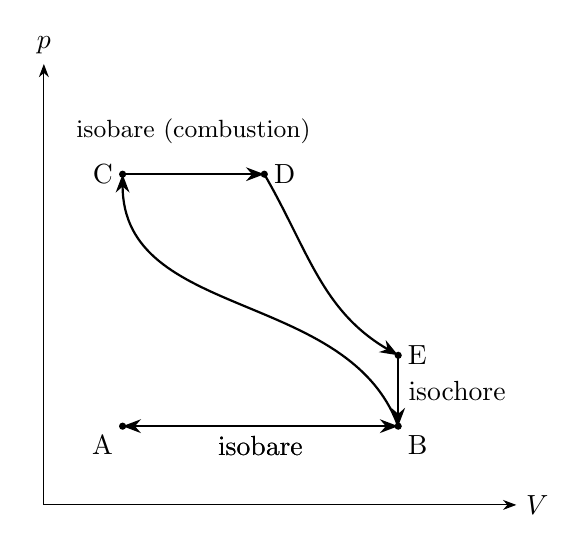
\begin{tikzpicture}[scale=1, >=Stealth]
\draw[->] (0,0) -- (6,0) node[right] {$V$};
\draw[->] (0,0) -- (0,5.6) node[above] {$p$};
\coordinate (A) at (1,1); \coordinate (B) at (4.5,1);
\coordinate (C) at (1,4.2); \coordinate (D) at (2.8,4.2);
\coordinate (E) at (4.5,1.9);
\draw[thick,->] (A) -- (B) node[midway,below]{isobare};
\draw[thick,->] (B) to[out=110,in=-90] (C);
\draw[thick,->] (C) -- (D);
\node at (1.9,4.75) {\small isobare (combustion)};
\draw[thick,->] (D) to[out=-60,in=150] (E);
\draw[thick,->] (E) -- (B) node[midway,right]{isochore};
\draw[thick,dashed,->] (B) -- (A) node[midway,below]{isobare};
\foreach \p/\lab/\pos in {A/A/below left,B/B/below right,C/C/left,D/D/right,E/E/right}
  {\fill (\p) circle (1.3pt) node[\pos] {\lab};}
\end{tikzpicture}
\end{center}

\subsection*{Calcul du rendement (diffère de l'essence à cause de la combustion isobare)}
\begin{demotable}
$\eta=1+\dfrac{Q_{EB}}{Q_{CD}}=1+\dfrac{nC_v(T_B-T_E)}{nC_p(T_D-T_C)}$ &
Comme pour l'essence, mais $Q_{CD}$ utilise maintenant $C_p$ car la combustion C-D est \textbf{isobare} (et
non plus $C_v$). \\
On définit $\rho=\dfrac{V_D}{V_C}$ (rapport de combustion, ou d'injection), en plus de
$\varepsilon=\dfrac{V_B}{V_C}$ &
$\rho$ mesure de combien le volume augmente pendant l'injection/combustion à pression constante (nouveau
paramètre, absent chez l'essence où $V_D=V_C$). \\
Adiabatiques B-C et D-E, plus la relation isobare $T_D/T_C=V_D/V_C=\rho$ &
Mêmes outils que pour l'essence, en ajoutant la loi des gaz parfaits appliquée à l'isobare C-D. \\
\end{demotable}
\eqbox{\eta_{\text{théorique}}=1+\dfrac{\varepsilon^{1-\gamma}-\varepsilon^{1-\gamma}\cdot\rho^{\gamma}}
{\gamma(\rho-1)}}
\emph{En mots :} le rendement théorique du diesel dépend de \textbf{deux} paramètres géométriques
($\varepsilon$ et $\rho$) au lieu d'un seul pour l'essence -- logique, puisque la combustion diesel n'est
plus instantanée mais s'étale sur une phase isobare caractérisée par $\rho$. Les rendements de forme,
mécanique et effectif se calculent \textbf{exactement de la même façon} que pour l'essence.

\newpage
\section{Moteur 2 temps : phases, comparaison avec le 4 temps (diapos 177-182)}

\begin{objectif}
\textbf{Pas de nouvelle démonstration ici} : le cycle thermodynamique idéal est le \textbf{même} que celui
de l'essence (compression adiabatique, combustion isochore, détente adiabatique, échappement) -- donc
\textbf{même formule} $\eta_{\text{théorique}}=1-\varepsilon^{1-\gamma}$. Ce qui change, c'est la
\textbf{mécanique}.
\end{objectif}

\begin{demotable}
Pas de soupapes : deux ouvertures (\textbf{lumières}) dégagées ou bouchées par le piston lui-même &
Plus simple mécaniquement : le piston fait à la fois office de piston et de «distributeur» pour
l'admission/échappement. \\
\textbf{1 tour du moteur = 1 cycle complet} (au lieu de 2 tours en 4 temps) &
Tout se passe en une seule remontée-descente du piston : combustion+détente+échappement+admission se
chevauchent en un seul temps, puis compression dans l'autre. \\
Temps 1 : combustion, détente, échappement \textbf{et} admission simultanés &
Le mélange explose, le piston descend et découvre les lumières : les gaz brûlés sortent pendant que le
mélange neuf entre en même temps (balayage). \\
Temps 2 : compression, pendant que le mélange neuf est aspiré dans le carter &
Le piston remonte et comprime le mélange dans le cylindre, tandis qu'en dessous, le carter aspire déjà le
mélange du \textbf{prochain} cycle. \\
\end{demotable}

\begin{center}
\renewcommand{\arraystretch}{1.5}
\begin{tabularx}{\linewidth}{@{}>{\raggedright\arraybackslash}X >{\raggedright\arraybackslash}X@{}}
\toprule
\textbf{Avantages (vs 4 temps)} & \textbf{Inconvénients (vs 4 temps)} \\
\midrule
À cylindrée égale, puissance plus importante & Bruyant \\
Pour un cylindre, couple moteur plus régulier & Une partie de l'essence passe par l'échappement sans être
brûlée $\Rightarrow$ rendement plus faible \\
Organes simplifiés, moins lourd & Réglage des lumières compliqué \\
\bottomrule
\end{tabularx}
\end{center}

\begin{retenir}
\textbf{Puissance :} $P_{eff}=\dfrac{N}{60}\cdot W_{dispo}\cdot z$ -- \textbf{pas de division par 2} car 1
tour = 1 cycle (contrairement au 4 temps où $P=\frac{N}{2\cdot60}W\cdot z$). C'est le piège classique
à l'examen sur cette matière. Usages typiques : deux-roues, tondeuses -- machines compactes et légères.
\end{retenir}

\newpage
\section{Entropie : théorème de Carnot généralisé, réversible/irréversible (diapos 189-192)}

\begin{objectif}
\textbf{Objectif :} généraliser à un nombre quelconque de sources ce qu'on a vu avec Carnot (2 sources), et
définir une grandeur -- l'entropie -- qui permet de savoir si une transformation est possible et si elle est
réversible ou non.
\end{objectif}

\subsection*{Théorème de Carnot généralisé (diapo 189)}
\begin{demotable}
Cas réversible : $\displaystyle\sum\frac{Q_i}{T_i}=0 \Rightarrow \int\frac{dQ}{T_{sources}}=0$ &
En généralisant le résultat de Carnot (2 sources, $Q_1/T_1+Q_2/T_2=0$ à la limite réversible) à un nombre
quelconque $n$ de sources. \\
Cas irréversible : $\displaystyle\sum\frac{Q_i}{T_i}<0 \Rightarrow \int\frac{dQ}{T_{sources}}<0$ &
En irréversible, cette somme n'est plus nulle mais toujours \textbf{négative} (jamais positive). \\
\end{demotable}

\subsection*{Notion d'entropie -- cas réversible (diapo 190)}
\begin{demotable}
Deux chemins réversibles I et II entre A et B : $\displaystyle\int_I\frac{dQ}{T}-\int_{II}\frac{dQ}{T}=0$ &
On applique le théorème ci-dessus au cycle fermé formé par l'aller (I) et le retour (II), tous deux
réversibles $\Rightarrow$ la somme totale vaut $0$. \\
$\displaystyle\int_I\frac{dQ}{T}=\int_{II}\frac{dQ}{T}=\boxed{\Delta S}$ &
Cette quantité est donc \textbf{la même quel que soit le chemin réversible suivi} entre A et B : c'est une
fonction d'état, qu'on appelle l'\textbf{entropie} $S$, échangée entre le système et l'extérieur. \\
\end{demotable}

\subsection*{Cas où I est réversible et II irréversible (diapo 191)}
\begin{demotable}
$\displaystyle\int_I\frac{dQ}{T}-\int_{II}\frac{dQ}{T}<0$ &
Même raisonnement, mais le cycle contient maintenant une partie irréversible (II) : le théorème de Carnot
donne cette fois une inégalité stricte. \\
$\displaystyle\int_I\frac{dQ}{T}<\int_{II}\frac{dQ}{T}<\Delta S_{irrev}$ &
On note $\Delta S_{irrev}=\int_{II}dQ/T$ le long du chemin irréversible : il est \textbf{plus grand} que
l'intégrale réversible. \\
$\displaystyle\int_I\frac{dQ}{T}+\Delta S_i=\Delta S_{irrev}$, où $\Delta S_i>0$ &
On introduit $\Delta S_i$, l'\textbf{entropie créée} par les irréversibilités (frottements, pertes...),
pour transformer l'inégalité en égalité. \\
\end{demotable}

\begin{retenir}
\textbf{Système isolé} ($dQ=0$, aucun échange avec l'extérieur) : l'entropie \textbf{reste constante} si la
transformation est réversible, et \textbf{augmente} si elle est irréversible ($\Delta S_i>0$ toujours). C'est
le sens physique du second principe : l'univers évolue toujours vers plus de désordre
($S=k_b\ln\Omega$, $\Omega$ = nombre d'états microscopiques possibles).
\end{retenir}

\subsection*{Calculer une variation d'entropie en pratique (diapo 194)}

Pour une transformation \textbf{réversible}, on part de $\displaystyle\Delta S=\int\frac{dQ}{T}$ et on
remplace $dQ$ selon le type de transformation :

\begin{demotable}
\textbf{À pression constante} : $dQ=nC_p\,dT$, donc
$\Delta S=\displaystyle\int\frac{nC_p\,dT}{T}=\boxed{nC_p\ln\!\left(\frac{T_2}{T_1}\right)}$ &
On injecte $dQ=nC_p\,dT$ (isobare) dans l'intégrale ; $\int\frac{dT}{T}=\ln T$, d'où le logarithme du
rapport des températures. \\
\textbf{À volume constant} : $dQ=nC_v\,dT$, donc
$\Delta S=\boxed{nC_v\ln\!\left(\frac{T_2}{T_1}\right)}$ &
Même calcul, mais avec $C_v$ puisque la transformation est isochore. \\
\textbf{À température constante} : $\Delta U=0$ donc $Q=-W$, et $T$ sort de l'intégrale :
$\Delta S=\dfrac{1}{T}\displaystyle\int -dW=\boxed{nR\ln\!\left(\frac{V_2}{V_1}\right)}$ &
Sur une isotherme, $T$ étant constante on peut la sortir de $\int\frac{dQ}{T}$ ; il reste
$\frac{Q}{T}$, et $Q=-W=nRT\ln\frac{V_2}{V_1}$ (travail isotherme, section 1). \\
\textbf{Adiabatique réversible} : $dQ=0$ donc $\boxed{\Delta S=0}$ &
C'est pour cela qu'on l'appelle aussi \textbf{isentropique} : pas de chaleur échangée \emph{et} pas
d'irréversibilité $\Rightarrow$ l'entropie ne bouge pas. \\
\end{demotable}

\begin{retenir}
\textbf{Sur un cycle complet, $\Delta S=0$} (l'entropie est une fonction d'état, on revient au point de
départ) : c'est une vérification supplémentaire, au même titre que $\Delta U=0$. Attention, cela ne veut
pas dire que l'entropie \emph{créée} $\Delta S_i$ est nulle : si le cycle est irréversible, il en a été
créé, mais elle a été évacuée vers l'extérieur avec la chaleur.
\end{retenir}

\newpage
\section{Machine frigorifique : schéma et diagramme $\log p$-$h$ (diapos 251-256)}

\textbf{Principe :} un frigo/PAC est un \textbf{cycle récepteur} à deux sources (il faut fournir un travail
$W>0$). La vapeur passe dans un compresseur (p et T augmentent), puis dans un condenseur au contact de la
source chaude (elle cède de la chaleur et se liquéfie), puis dans une soupape de détente (p et T chutent),
puis dans un évaporateur au contact de la source froide (elle reçoit de la chaleur et se vaporise).

\begin{demotable}
$1\to2$ : \textbf{compression isentropique} &
La vapeur passe dans le compresseur ; si $p$ augmente, $T$ augmente aussi. Réversible $\Rightarrow$ entropie
constante. \\
$2\to3$ : \textbf{condensation isobare}, dans le condenseur, au contact de la source chaude &
La vapeur comprimée est plus chaude que la source chaude : elle lui cède de l'énergie et se condense (le
système donne $Q_1<0$). \\
$3\to4$ : passage dans la \textbf{soupape de détente}, à \textbf{enthalpie constante} &
Aucune pièce mobile n'échange de travail utile ($W_{ut}=0$) et la détente est trop rapide pour échanger de
la chaleur ($Q=0$) $\Rightarrow$ d'après le 1\textsuperscript{er} principe en machine ouverte
($\Delta H=W_{ut}+Q$), on a $\Delta H=0$. \\
$4\to1$ : \textbf{évaporation isobare}, dans l'évaporateur, au contact de la source froide &
Le liquide (froid, basse pression) est plus froid que la source froide : il peut donc en recevoir de la
chaleur $Q_2>0$ et s'évaporer. \\
\end{demotable}

\textbf{Le diagramme des frigoristes $(\log p,h)$} : les fluides utilisés sont \textbf{organiques} (liaisons
covalentes, plus fortes que les liaisons ioniques $\Rightarrow$ plus d'énergie de vaporisation nécessaire,
cloche de saturation plus large). On place les 4 points \textbf{réels} $1',2',3',4'$ avec une
\textbf{surchauffe} ($\sim5\,^\circ$C au-dessus de $T_{\text{évap}}$ en 1') pour garantir un gaz sec, et un
\textbf{sous-refroidissement} ($\sim5\,^\circ$C sous $T_{cond}$ en 3') pour garantir du liquide pur -- cela
limite les irréversibilités.

\begin{retenir}
Pour $1\to2$ réel (non isentropique), le rendement isentropique du compresseur relie le point idéal
(isentropique) au point réel : $\displaystyle\eta_{isos}=\frac{h_{2\,\text{isos}}-h_1}{h_{2\,\text{réel}}-h_1}$. $T_{2'}$
et $T_{3'}$ doivent rester \textbf{au-dessus} de la température de la source chaude (sinon pas d'échange de
chaleur possible vers elle) ; $T_{1'}$ et $T_{4'}$ doivent rester \textbf{en dessous} de celle de la source
froide.
\end{retenir}

\section{PSN, COP, rendement de Carnot pour un frigo/PAC (diapos 257-263)}

\begin{demotable}
Frigo : $\boxed{PSN=\dfrac{Q_2}{W}}$ &
L'énergie «utile» d'un frigo, c'est la chaleur \textbf{prise} à la source froide (l'intérieur du
frigo). On la rapporte au travail qu'il a fallu fournir. \\
PAC : $\boxed{COP=\dfrac{-Q_1}{W}}$ &
Pour une pompe à chaleur, l'énergie utile est la chaleur \textbf{cédée} à la source chaude (l'intérieur de
la maison) ; $Q_1<0$ donc on met un signe $-$ pour que le $COP$ soit positif. \\
\end{demotable}

\subsection*{Démonstration de $PSN_{max}$ et $COP_{max}$ (cycle réversible)}
\begin{demotable}
$Q_1+Q_2+W=\Delta U=0$ (bilan sur un cycle) &
Comme pour tout cycle fermé, l'énergie interne revient à sa valeur de départ : la somme de tout ce qui
entre/sort vaut $0$. \\
Si le cycle est réversible : $\dfrac{Q_1}{T_1}+\dfrac{Q_2}{T_2}=\Delta S=0 \Rightarrow
\boxed{\dfrac{Q_1}{Q_2}=-\dfrac{T_1}{T_2}}$ &
On applique le résultat de la section «entropie» : à la limite réversible, l'entropie totale
échangée avec les 2 sources est nulle. \\
$PSN_{max}=\dfrac{Q_2}{-Q_1-Q_2}=\dfrac{1}{-(Q_1/Q_2)-1}=\dfrac{1}{(T_1/T_2)-1}$ &
On remplace $W=-Q_1-Q_2$ (issu du bilan) dans $PSN=Q_2/W$, on divise haut et bas par $Q_2$, puis on
substitue le rapport $Q_1/Q_2=-T_1/T_2$ trouvé juste avant. \\
$\boxed{PSN_{max}=\dfrac{T_2}{T_1-T_2}}$ &
On multiplie haut et bas par $T_2$ pour simplifier la fraction. \\
\midrule
$COP_{max}=\dfrac{-Q_1}{-Q_1-Q_2}=\dfrac{1}{(Q_2/Q_1)+1}=\dfrac{1}{(-T_2/T_1)+1}$ &
Même méthode pour la PAC : on remplace $W=-Q_1-Q_2$ dans $COP=-Q_1/W$, on divise haut et bas par $Q_1$ cette
fois, puis on substitue $Q_2/Q_1=-T_2/T_1$ (inverse de la relation précédente). \\
$\boxed{COP_{max}=\dfrac{T_1}{T_1-T_2}}$ &
On multiplie haut et bas par $T_1$. Notez que $COP_{max}=PSN_{max}+1$ : logique, car $COP$ compte
\emph{toute} l'énergie cédée à la source chaude (chaleur prise au froid \emph{plus} le travail fourni),
alors que $PSN$ ne compte que la chaleur prise au froid. \\
\end{demotable}

\begin{retenir}
$T_1$ et $T_2$ dans ces formules sont les \textbf{températures des sources réelles} (air extérieur, air
ambiant, eau du circuit...), en \textbf{Kelvin} -- pas les températures d'évaporation/condensation du fluide
frigorigène (qui sont décalées à cause de l'écart d'échange). Ces bornes $PSN_{max}$/$COP_{max}$ ne sont
jamais atteintes en pratique (compression non isentropique, surchauffe, sous-refroidissement...).
\end{retenir}


\end{document}
